% !TeX root = ../main.tex
\chapter{Introduction}

\lettrine{W}{e} start by looking at examples which demonstrate some of the motives behind studying analysis in general.
%
\begin{example*}[Series]
  The geometric series
  \(S = 1 + \frac{1}{2} + \frac{1}{4} + \frac{1}{8} + \frac{1}{16} + \cdots\)
  can be summed by the following simple trick.
  Multiplying by \(2\) we obtain that
  \[
    2S = 2 + 1 + \frac{1}{2} + \frac{1}{4} + \frac{1}{8} + \frac{1}{16} + \cdots = 2+S
  \]
  and so \(S=2\).
  If we try to do the same to the sum
  \(T = 1 + 2 + 4 + 8 + 16 + \cdots\)
  we get the nonsensical answer
  \[
    2T = 2 + 4 + 8 + 16 + \cdots = T -1
  \]
  and so \(T = -1\).
  %
  Why should we trust the argument in the first case and not in the second?
\end{example*}


\begin{example*}[Interchanging sums]
  If we consider any matrix of numbers, for example,
  \[
    \begin{pmatrix}
      1 & 2 & 3 \\
      4 & 5 & 6 \\
      7 & 8 & 9
    \end{pmatrix}
  \]
  we can sum first the rows \(6 + 15 + 24 = 45\) or first the columns \(12 + 15 + 18 = 45\) to obtain the total sum of all numbers.
  This is the rule
  \[
    \sum_{j=1}^{m} \sum_{k=1}^{n} a_{jk} = \sum_{k=1}^{n} \sum_{j=1}^{m}  a_{jk}.
  \]
  We would like to believe that also \(\sum_{j=1}^{\infty} \sum_{k=1}^{\infty} a_{jk} = \sum_{k=1}^{\infty} \sum_{j=1}^{\infty}  a_{jk}\).
  However this doesn't work for the following matrix:
  \[
    \begin{pmatrix}
      1      & 0      & 0      & \cdots \\
      -1     & 1      & 0      & \cdots \\
      0      & -1     & 1      & \cdots \\
      \vdots & \vdots & \vdots & \ddots
    \end{pmatrix}.
  \]
  %
  We often want to swap the order of summing (or integrating) and often need to consider infinite sums (or integrals).
  When can we do this and can't we?
\end{example*}

\begin{example*}[Interchanging integrals]
  Let's try to integrate \(e^{-xy} - xye^{-xy}\) with respect to both \(x\) and \(y\).
  We would like to believe that
  \[
    \int_{0}^{\infty} \left[ \int_{0}^{1} (e^{-xy} - xye^{-xy}) \ dy \right] \ dx
    \overset{\text{\large\color{blue}?}}{=} \int_{0}^{1} \left[ \int_{0}^{\infty}  (e^{-xy} - xye^{-xy}) \ dx \right] \ dy.
  \]
  Since
  \( \int_{0}^{1} (e^{-xy} - xye^{-xy}) \ dy = {\left[ye^{-xy}\right]}_{y=0}^{1} = e^{-x}\),
  the left-hand side is
  \( \int_{0}^{\infty} e^{-x} \ dx = {\left[ -e^{-x} \right]}_{0}^{\infty} = 1 \).
  However, since
  \( \int_{0}^{\infty}  (e^{-xy} - xye^{-xy}) \ dx = {\left[ xe^{-xy} \right]}_{x=0}^{\infty} = 0\),
  the right-hand side is \(\int_{0}^{1} 0 \ dx = 0\).
  So how do we know when to trust the interchange of intervals?
\end{example*}


\begin{example*}[interchanging limits]
  We could easily believe that
  \[
    \lim_{x\to 0}\lim_{y\to 0} \frac{x^2}{x^2 + y^2}
    \overset{\text{\large\color{blue}?}}{=}
    \lim_{y\to 0}\lim_{x\to 0} \frac{x^2}{x^2 + y^2}.
  \]
  However \(\lim_{y\to 0} \frac{x^2}{x^2 + y^2} = \frac{x^2}{x^2 + 0} = 1 \) and so the left-hand side is \(1\)
  whereas \(\lim_{x\to 0} \frac{x^2}{x^2 + y^2} = \frac{0}{0 + y^2} = 0\) so the right-hand side is \(0\).
  What does the graph of this function look like?
  This example shows that the interchange of limits is untrustworthy. Under what circumstances is it legitimate?
\end{example*}

We need to be rigorous in our logic otherwise, as we have seen in these examples, the conclusions can be erroneous and the difficulties are often subtle.

\subsection*{Curves of constant width}
%
\begin{figure}[htb]
  \centering
  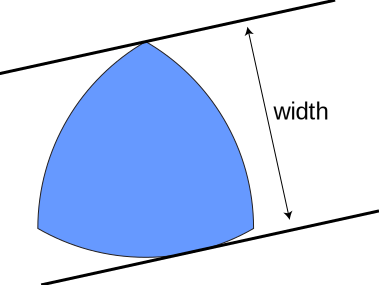
\includegraphics{reuleaux.pdf}
  \caption{The Reuleaux triangle is a curve of constant width.}%
  \label{fig:reuleaux}
\end{figure}
%
The above examples are calculus based but it is worthwhile to consider a real world application of the rigour and reasoning we aspire to.
Suppose we are organising the production facilities which manufacture a component that is round (maybe a rocket body, maybe a propellant tube, etc.).
\begin{samepage}
  As part of the production it is important to have a procedure which guarantees that the fabrication is done to the correct tolerance.
  The idea proposed is:
  \begin{quotation}
    ``We measure the width from all angles to confirm that the manufactured component is correct.''
  \end{quotation}
\end{samepage}
This is a two-dimensional problem in the sense we assume that the object is a closed curve in \(\bR^2\).
For a given angle we define the width of this curve to be the smallest distance between two parallel lines which touch the curve in a single point but never cross it (one each side of the curve).
We say that the curve has constant width if this width is equal from every direction.
This is just what we would check using calipers on a part and rotating.
The following statement is intuitive and true.
\begin{theorem*}
  A circle has constant width.
\end{theorem*}
\noindent
However the converse is not true, indeed the following is true.
\begin{theorem*}
  There exist constant width curves which are not circles.
\end{theorem*}
\noindent
This can be proved by constructing many such curves, for example the \href{https://en.wikipedia.org/wiki/Reuleaux_triangle}{Reuleaux triangle}. Indeed there are such curves which look similar to regular polygons but still have constant width.


% \footnotetext{
%   Source of Figure~\ref{fig:reuleaux}: 
%   \url{https://commons.wikimedia.org/wiki/File:Reuleaux_supporting_lines.svg}
%   }



\subsection*{MA2 versus MA1}

Much of what we do in this course builds on ideas established in Mathematical Analysis 1.
In particular many of the ideas are extended to the higher dimensional setting. See Table~\ref{tab:2versus1}.

\begin{table}
  \centering
  \begin{tabular}{r | l} % chktex 44
    \textbf{Mathematical Analysis 1}
     &
    \textbf{Mathematical Analysis 2}  \\
    \midrule
    Sequences \& series of numbers
     &
    Sequences \& series  of functions \\
    \(a_1, a_2, a_3,\ldots \)
     &
    \(f_1(x), f_2(x), f_3(x),\ldots \)
    \\
    \(\sum_{n=0}^{\infty} a_n\)
     &
    \(\sum_{n=0}^{\infty} f_n(x)\)
    \\
    \midrule
    (Functions) \(f:\bR \to \bR\)
     &
    \(f:\bR^n \to \bR\) (Scalar fields)
    \\
     &
    \(\mathbf{f}:\bR^n \to \bR^n\) (Vector fields)
    \\
     &
    \(\boldsymbol{\alpha}:\bR \to \bR^n\) (Paths)
    \\
    \midrule
    (Derivative) \( f'(x) = \frac{df}{dx}(x)\)
     &
    \( \frac{\partial f}{\partial x_j}(x_1,\ldots,x_n)\) (Partial derivatives)
    \\
     &
    \(\nabla f\) (Gradient)
    \\
     &
    \(D_v f\) (Directional derivative)
    \\
     &
    \(\boldsymbol{\alpha}'\) (Derivative of path)
    \\
     &
    \(Df\) (Jacobian matrix)
    \\
     &
    \(\nabla \cdot \ff\) (Divergence)
    \\
     &
    \(\nabla \times \ff\) (Curl)
    \\
    \midrule
    (Extrema) \(\sup_{x\in \bR} f(x)\)
     &
    \(\sup_{x\in \bR^n} f(x)\) (Extrema)
    \\
     &
    Lagrange multiplier method
    \\
    \midrule
    Integral \(\int_{a}^{b} f(x) \ dx\)
     &
    Multiple integral
    \\
     &
    Line integral
    \\
     &
    Surface integral
  \end{tabular}
  \caption{Ma2 versus MA1}%
  \label{tab:2versus1}
\end{table}

\subsection*{A brief review of MA1}
In MA1, we learnt some properties of real numbers $\bR$, functions defined on subsets of $\bR$
and operation on them such as differentiation and integration.

\subsubsection*{Real numbers}
On the set of real numbers there are operations $+$ (sum) and $\cdot$ (product), and the order $<$.
We say that a subset $A \subset \bR$ is bounded above if there is $a \in \bR$ such that,
for any $x \in A$, it holds that $x \le a$. Similarly, we say that $A$ is bounded below if there is $a \in \bR$
such that, for any $x \in A$, it holds that $a \le x$. We say that $A$ is bounded if $A$ is bounded both above and below.
We assumed that, for any bounded $A$, there is the smallest upper bound $\sup A \in \bR$.

\subsubsection*{Sequences and functions}

We say that a sequence $\{a_n\}$ of real numbers converges to $a \in \bR$ if, for any $\epsilon > 0$,
there is $N$ such that $|a_n - a| < \epsilon$ for $n \ge N$. In this case, we denote $a_n \to a$ or $\lim_{n\to \infty}a_n = a$.
We learnt that, if $\{a_n\}$ is a bounded sequence, then there is a convergent subsequence.

A function $f$, defined on $A \subset \bR$, is an assignment of a (real) number $f(x)$ to each $x \in A$.
Let $x_0 \in A$. We say that $f$ is continuous at $x_0$ if for any sequence $\{x_n\} \subset A$ such that $x_n \to x_0$,
it holds that $f(x_n) \to f(x_0)$. We say simply that $f$ is continuous if $f$ is continuous at every point $x \in A$.

\subsubsection*{Differentiation}

Let $f$ be a function defined on an open interval $I$ and let $x_0 \in I$.
We say that $f$ is differentiable at $x_0$ if the limit
\begin{align*}
 \lim_{h\to \infty} \frac{f(x_0 + h) - f(x_0)}h
\end{align*}
exists, and denote it $f'(x_0)$, or $\frac{df}{dx}(x_0)$, and call it the derivative of $f$ at $x_0$.
If $f$ is differentiable at all points in $I$, then the assignment $x \mapsto f'(x)$ is a new function,
called the derivative of $f$. For concrete functions,
\begin{itemize}
 \item If $f(x) = x^n$, then $f'(x) = nx^{n-1}$.
 \item If $f(x) = e^x$, then $f'(x) = e^x$.
 \item If $f(x) = \log x$, then $f'(x) = \frac1x$.
 \item If $f(x) = \sin x$, then $f'(x) = \cos x$.
 \item If $f(x) = \cos x$, then $f'(x) = -\sin x$.
\end{itemize}
If $f(x) > 0$ (respectively $f(x) < 0$) in an open interval $I$, then $f$ is monotonically increasing (respectively decreasing) on $I$.

\subsubsection*{Integration}

We also defined the integral of (continuous) functions using the Riemann sum.
By the fundamental theorem of calculus, it holds that 
$\frac{d}{dx}\int_a^x f(t)dt = f(x)$, and if $F'(x) = f(x)$, then $\int_a^b f(t)dt = F(b)-F(a)$.
We can calculate many integrals using the known derivatives.

\subsection*{Remarks about logic and sets}
We studied that we can write mathematical statements about real numbers.
Often these statements come with ``for all $x$ ... it holds that...'' or ``there exist $x$... such that...''.
(We can write these statements using the symbols $\forall, \exists$).
They are called quantifiers, and it means that we are not talking about a number called $x$, but it is talking about
all numbers or the existence of some numbers with the specified properties.

Let us recall that the negation of a statement with a quantifiers is equivalent to a statement with the other quantifier.
For example,
\begin{itemize}
 \item The negation of ``for all real number $x$, it holds that $x > 0$''
 is ``there exist a real number $x$ such that not $x > 0$'',
 that is, ``there exist a real number $x$ such that not $x \le 0$'',
 and this is a true statement, because there are negative numbers such as $-1$.
 \item The negation of ``there exist a real number $x$ such that $10 < x$''
 is ``for all real number $x$, it does not hold that $10 < x$'',
 that is,  ``for all real number $x$, $10 \ge x$''. This is false, because we can take $x=11$.
\end{itemize}


The order of quantifiers is important. For example,
\begin{itemize}
 \item Consider the statement ``For any real number $x$, there is a real number $y$ such that $x < y$.''
 This is a true statement. Indeed, for any real number $x$, we can take $y = x + 1$.
 \item The statement ``There is a real number $y$ such that, for any real number $x$, it holds that $x < y$ is false.
 Indeed, for any $y$, $y < y+1$, thus the conclution $y+1 < y$ is false, and the whole statement is false.
\end{itemize}




\subsection*{Suggested further reading}

\begin{itemize}
  \item ``Analysis 1'' by Terence Tao.
        (Particularly \S 1.2 ``Why Analysis?'' and Appendix A ``The basics of mathematical logic'').
\end{itemize}

\bookletend%
